\documentclass[xcolor=table]{beamer}
%\documentclass[handouts]{beamer}
%\setbeameroption{show notes}
\setbeameroption{hide notes}
%\setbeameroption{show only notes}


%[xetex,mathserif,serif]
\usepackage{multicol}
%\usepackage{animate}
\usepackage{verbatim}
\makeatletter
\newcommand{\verbatimfont}[1]{\renewcommand{\verbatim@font}{\ttfamily#1}}
\makeatother
\usepackage{hyperref}
\usepackage{tikz}

\graphicspath{{images/}}

%KTH official colors https://intra.kth.se/polopoly_fs/1.486828!/image/fargreferens_png.png
\definecolor{kthBlue}{RGB}{25,84,166} %Bla
\definecolor{kthLightBlue}{RGB}{36,160,216} %Ljusbla

\definecolor{kthRed}{RGB}{157,16,45} %Rod
\definecolor{kthLigthRed}{RGB}{228,54,62} %Lujsrod

\definecolor{kthGrey}{RGB}{101,101,108} %Morkgra
\definecolor{kthLightGrey}{RGB}{227,229,227} %Ljusgra
\definecolor{kthMediumGrey}{RGB}{189,188,188} %Mellangra

\definecolor{kthGreen}{RGB}{98,146,46} %Gorn
\definecolor{kthLightGreen}{RGB}{176,201,43} %Ljusgron


\usetheme{AnnArbor}

% \setbeamercolor{background canvas}{bg=white}
\setbeamercolor*{structure}{fg=kthLightBlue,bg=kthBlue}
\setbeamercolor*{palette primary}{use=structure,fg=white,bg=kthBlue} 
\setbeamercolor*{palette secondary}{use=structure,fg=black,bg=kthLightGrey}
\setbeamercolor*{palette tertiary}{use=structure,fg=black,bg=kthLightBlue}
%\setbeamercolor*{palette quaternary}{use=structure,fg=black,bg=kthLightGrey}


\setbeamercolor*{frametitle}{fg=kthBlue,bg=kthLightGrey}
\setbeamercolor*{alerted text}{fg=kthRed}
\setbeamercolor*{item projected}{fg=white,bg=kthLightBlue}
%\setbeamercolor{palette sidebar primary}{use=structure,fg=structure.fg,bg=red}
%\setbeamercolor{palette sidebar secondary}{use=structure,fg=structure.fg,bg=green}
%\setbeamercolor{palette sidebar tertiary}{use=normal text,fg=normal text.fg}


\setbeamercolor{block title}{bg=kthMediumGrey}
\setbeamercolor{block body}{bg=normal text.bg!90!black}

\setbeamercolor{block title alerted}{use={normal text,alerted text},fg=alerted text.fg!75!normal text.fg,bg=normal text.bg!75!black}
\setbeamercolor{block body alerted}{bg=normal text.bg!90!black}

\setbeamercolor{block title example}{use={normal text,example text},fg=example text.fg!75!normal text.fg,bg=normal text.bg!75!black}
\setbeamercolor{block body example}{bg=normal text.bg!90!black}

%\setbeamercolor{fine separation line}{}
%\setbeamercolor{normal text}{bg=white,fg=black}
%\setbeamercolor{section in sidebar}{fg=red}
%\setbeamercolor{section in sidebar shaded}{fg=grey}
%\setbeamercolor{separation line}{}
%\setbeamercolor{structure}{bg=black, fg=kthGreen}
%\setbeamercolor{subsection in sidebar}{fg=brown}
%\setbeamercolor{subsection in sidebar shaded}{fg=grey}
\setbeamercolor{title}{fg=white,bg=kthBlue}
%\setbeamercolor{titlelike}{fg=DarkGreen}


%\setbeamercolor{sidebar}{bg=red}
%\setbeamercolor{sidebar}{parent=palette primary}
%\setbeamercolor{palette sidebar primary}{fg=red}%use=normal text,fg=normal text.fg}
%\setbeamercolor{palette sidebar quaternary}{fg=red}
%\setbeamercolor{palette sidebar secondary}{use=structure,fg=structure.fg}
%\setbeamercolor{palette sidebar tertiary}{use=normal text,fg=normal text.fg}



\title{Introduction to PDC environment}
\subtitle{}

%\author{Thor Wikfeldt}
%\author{Xin Li}
%\author{Tor Kjellsson Lindblom}
\author{Johan Hellsvik}

\institute[PDC]{
  PDC Center for High Performance Computing\\
  KTH Royal Institute of Technology
  }
  \logo{
   \includegraphics[width=1cm,keepaspectratio]{logo_kth_transparent}~%
   % \includegraphics[width=1cm,height=1cm,keepaspectratio]{logo_kth+pdc_blue}~%
 
}
%\date[PDC Oct 2017]{Introduction to PDC, February 2018}
%\date[PDC Aug 2019]{PDC Summer School August 2019}
%\date[PDC Jan 2021]{Introduction to PDC, January 2021}
%\date[PDC Apr 2021]{Introduction to PDC, April 2021}
\date[PDC Apr 2021]{Introduction to PDC, September 2021}  
\subject{Introduction}


\begin{document}
\frame{\titlepage}

\AtBeginSection[]
{
  \begin{frame}
    \frametitle{Outline}
    \tableofcontents[currentsection]
  \end{frame}
}
%\AtBeginSubsection[]
%{
 % \begin{frame}
  %  \frametitle{Table of Contents}
   % \tableofcontents[currentsection,currentsubsection]
 % \end{frame}
%}

%\frame[plain]{
%Large image inclusion 
%\color{kthBlue}{kthBlue}\\
%\color{kthLightBlue}{kthLightBlue}\\
%\color{kthRed}{kthRed}\\
%\color{kthLigthRed}{kthLigthRed}\\
%\color{kthGrey}{kthGrey}\\
%\color{kthLightGrey}{kthLightGrey}\\
%\color{kthGreen}{kthGreen}\\
%\color{kthLightGreen}{kthLightGreen}\\
%\color{kthMediumGrey}{kthMediumGrey}
%}
%\frame[shrink]{
%%\begin{block}{Answered Questions}
%How many primes are there?
%\end{block}
%\begin{block}{Open Questions}
%Is every even number the sum of two primes?
%\end{block}
%}
%\frame[allowframebreaks]{
%The allowframebreaks option will auto-create new frames if there is too much content to be displayed on one.
%}



\newcommand\irregularcircle[2]{% radius, irregularity
  \pgfextra {\pgfmathsetmacro\len{(#1)+rand*(#2)}}
  +(0:\len pt)
  \foreach \a in {10,20,...,350}{
    \pgfextra {\pgfmathsetmacro\len{(#1)+rand*(#2)}}
    -- +(\a:\len pt)
  } -- cycle
}

\section{PDC Overview}
\subsection*{History}

\frame{
\frametitle{History of PDC}

\footnotesize
\begin{table}
\begin{tabular}{r|r|r|r|l|l} \hline 
\textbf{Year} & \textbf{rank} & \textbf{procs.} & \textbf{peak TFlops} & \textbf{vendor} & \textbf{name} \\ \hline
2017 & 69  & 67456 & 2438.1 & Cray & Beskow\footnote{XC40 16-core 2.3GHz} \\ \hline
2014 & 32  & 53632 & 1973.7 & Cray & Beskow \\ \hline
2011 & 31  & 36384 & 305.63 & Cray & Lindgren\footnote{XE6 12-core 2.1 GHz} \\ \hline
2010 & 76  & 11016 & 92.534 & Cray & Lindgren \\ \hline
2010 & 89  & 9800  & 86.024 & Dell & Ekman\footnote{PowerEdge SC1435 Dual core Opteron 2.2GHz, Infiniband} \\ \hline
2005 & 65  & 886   & 5.6704 & Dell & Lenngren\footnote{PowerEdge 1850 3.2 GHz, Infiniband} \\ \hline
2003 & 196 & 180   & 0.6480 & HP & Lucidor\footnote{Cluster Platform 6000 rx2600 Itanium2 900 MHz Cluster, Myrinet} \\ \hline
1998 & 60  & 146   & 0.0934 & IBM & Strindberg\footnote{SP P2SC 160 MHz} \\ \hline
1996 & 64  & 96    & 0.0172 & IBM & Strindberg \\ \hline
1994 & 341 & 256   & 0.0025 & Thinking Machines & Bellman\footnote{CM-200/8k} \\ \hline
\end{tabular}
\end{table}
}

\subsection*{Member of SNIC}

\frame
{
\frametitle{SNIC}
\framesubtitle{Swedish National Infrastructure for Computing}
\begin{columns}
\column{.3\textwidth}

\includegraphics[width=0.7\linewidth]{snic.png}\\
%\vspace{-55mm}
\column{.7\textwidth}
\footnotesize
National \alert{research infrastructure} that provides a \alert{balanced and cost-efficient} set of \alert{resources and user support} for \alert{large scale computation and data storage} to meet the needs of researchers from all scientific disciplines and from all over Sweden (universities, university colleges, research institutes, etc).\\
\hfill \break
SNIC is funded by the Swedish Research Council (VR-RFI) and the 10 participating universities: Chalmers, GU, KI, KTH, LiU, LU, SLU, SU, UmU, and UU.
\end{columns}
}

\subsection*{Business}
\frame{
\frametitle{Collaboration with industry}
\begin{columns}
\column{.5\textwidth}
  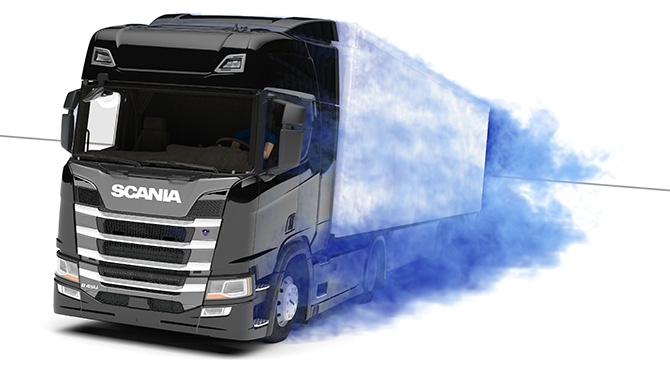
\includegraphics[width=\columnwidth]{Scania_truck}
\column{.5\textwidth}
\footnotesize
PDC's largest industrial partner is Scania. The figure shows a volume rendering of the instantaneous velocity magnitude on the leeward side of a Scania R20 Highline truck at crosswind conditions. (Source: Scania)
\end{columns}
\begin{itemize}
    \footnotesize
    \item Business partners \\
        \scriptsize
        \href{https://www.pdc.kth.se/research/business-research/pdc-partners}{https://www.pdc.kth.se/research/business-research/pdc-partners}
    \footnotesize
    \item White papers from research collaborations between PDC and European companies \\
        \scriptsize
        \href{https://www.pdc.kth.se/research/business-research/white-papers-1.737818}{https://www.pdc.kth.se/research/business-research/white-papers-1.737818}
    \footnotesize
    \item A small part of Dardel nodes will be dedicated to industry/business research.
    \item If you are interested in purchasing HPC compute time, contact PDC Support.
\end{itemize}
}

\subsection*{Training}
\frame{
  \frametitle{Broad Range of Training}
  \begin{description}
  \item [Summer School]
    Introduction to HPC held every year
  \item [Courses]
    \begin{itemize}
    %\item Programming for GPU
    \item Distributed and Parallel Computing
    \item Cloud Computing
    \item Programming for GPU
    \item Software Development Tools
    %\item CodeRefinery workshops
    \end{itemize}
  \item [PDC User Days] PDC Pub and Open House
  \end{description}
  \begin{columns}
    \column{.3\textwidth}
    \includegraphics[width=0.9\linewidth]{class3}
    \column{.3\textwidth}
    \includegraphics[width=0.9\linewidth]{class2}
    \column{.3\textwidth}
    \includegraphics[width=0.9\linewidth]{class1}
  \end{columns}
}

\subsection*{Staff}
\frame{
\frametitle{Support and System Staff}
\begin{exampleblock}{First-line support}
  Provide specific assistance to PDC users related to accounts, login, allocations etc.
\end{exampleblock}
\begin{exampleblock}{System staff}
  System managers/administrators ensure that computing and storage resources run smoothly and securely.
\end{exampleblock}
\begin{exampleblock}{Application Experts}
  Hold PhD degrees in various fields and specialize in HPC. Assist researchers in optimizing, scaling and enhancing scientific codes for current and next generation supercomputers.
\end{exampleblock}
}

\section{Infrastructure}

%\subsection*{Overview}
%\frame{
%\frametitle{What is a cluster?}
%\framesubtitle{\includegraphics[height=0.3\textheight,width=\textwidth]{Titan1}}
%
%\begin{columns}[T]
%\column{.4\textwidth}
%  \includegraphics[width=\columnwidth]{TitanIn}
%  \column{.3\textwidth}
%  \begin{itemize}
%    \item Cluster
%    \item Racks
%    \item Blades
%    \item Nodes
%    \item Processors 
%    \item Cores
%  \end{itemize}
%\column{.3\textwidth}
%  \begin{itemize}
%    \item Login nodes
%    \item Compute nodes
%    \item Dedicated nodes
%    \item Transfer nodes
%    \item Service nodes
%  \end{itemize}
%\end{columns}
%}


\subsection{Beskow}
\frame{
\frametitle{Beskow - Cray XC40 system}
\framesubtitle{\hspace{0.2\textwidth}\includegraphics[height=0.3\textheight]{Beskow}}

\begin{alertblock}{}{\alert{Fastest machine in Scandinavia}}\end{alertblock}

\begin{columns}
\column{.6\textwidth}
  \begin{itemize}
    \item Lifetime: Q3 2021
    \item $11$ racks, $2060$ nodes
    \item Intel Haswell processor 2.3 GHz \\ Intel Broadwell processor 2.1 GHz
    \item $67,456$ cores - $32$($36$) cores/node
    \item Aries Dragonfly network topology
    \item $156.4$ TB memory - $64$($128$) GB/node
  \end{itemize}
\column{.4\textwidth}
  \includegraphics[width=\columnwidth]{xc30-blade}
  \scriptsize\\
  $1$ XC compute blade\\
  $1$ Aries Network Chip ($4$ NICs)\\
  $4$ Dual-socket Xeon nodes\\
  $4$ Memory DIMM / Xeon node
\end{columns}
}

\subsection{Tegner}
\frame{
\frametitle{Tegner}
\framesubtitle{pre/post processing for Beskow}

\begin{columns}
\column{.4\textwidth}
\scriptsize
  \begin{alertblock}{$5$ x $2$~TB Fat nodes}
    $4$ x $12$ core Ivy Bridge, $2$~TB RAM \\
    $2$ x Nvidia Quadro K420
  \end{alertblock}
  
  \begin{alertblock}{$5$ x $1$~TB Fat nodes}
    $4$ x $12$ core Ivy Bridge, $1$~TB RAM \\
    $2$ x Nvidia Quadro K420
  \end{alertblock}
  
  \begin{alertblock}{$46$ Thin Nodes}
    $2$ x $12$ core Haswell, $512$~GB RAM \\
    Nvidia Quadro K420 GPU
  \end{alertblock}

  \begin{alertblock}{$9$ K80 Nodes}
    $2$ x $12$ core Haswell, $512$~GB RAM \\
    Nvidia Tesla K80 GPU
  \end{alertblock}

\column{.6\textwidth}
\normalsize
\centering\includegraphics[width=.5\columnwidth]{k420}
  
  \begin{itemize}
    \item Used for pre/post processing data 
    \item Has large RAM nodes
    \item Has nodes with GPUs
    \item Has two transfer nodes
    \item Lifetime: Q3 2021
  \end{itemize}
\end{columns}
}


\subsection*{Summary}
\frame{
\frametitle{Summary of PDC resources}
\framesubtitle{}
\begin{table}
  \begin{tabular}{r|l|l}
   & \alert{Beskow} & \alert{Tegner}\\ \hline \hline
  Cores in each node &  $32/36$ & $48/24$\\\hline
  Nodes &  $1676$ Haswell  & 55 x $24$ Haswell/GPU\\
        &  $384$ Broadwell & 10 x $48$ Ivy bridge\\\hline
  RAM (GB) & $1676$ x $64$~GB & $55$ x $512$~GB\\
           & $384$ x $128$~GB & $5$ x $1$~TB\\
           &                 & $5$ x $2$~TB\\\hline
  Allocations &&\\
  (core hours per month)&&\\
  Small &	$<5k$&	$<5k$\\
  Medium &	$<200k$&	$<80k$\\
  Large &	$\geq 200k$	 \\\hline
  Availability via SNIC &	yes &	with Beskow\\\hline
  AFS &	login node only &	yes\\
  Lustre &	yes	& yes\\
  \end{tabular}
\end{table}
}

\subsection*{File systems}
\frame{
\frametitle{File Systems}
\begin{block}{Andrew File System (\alert{AFS})}
\begin{itemize}
  \item Distributed file system accessible to any running AFS client
  \item Home directory \\  \url{/afs/pdc.kth.se/home/[initial]/[username]}
  \item Access via Kerberos tickets and AFS tokens
  \item \alert{Not accessible to compute nodes on Beskow}
\end{itemize}
\end{block}

\begin{block}{Lustre File System (\alert{Klemming})}
\begin{itemize}
 \item Open-source massively parallel distributed file system
 \item Very high performance ($5$~PB storage - $130$~GB/s bandwidth)
 \item NO backup (always move data when done), 25 GB personal quota
 \item Home directory \\  \url{/cfs/klemming/nobackup/[initial]/[username]}
\end{itemize}
\end{block}
}

\frame<presentation:0>[noframenumbering]{
\frametitle{File System Access}
 \begin{tabular}{ccc}
   
  \cellcolor{kthLightGreen} \textbf{AFS} & 
  \cellcolor{kthLightBlue}{Beskow Compute Node} &
  \cellcolor{kthLightBlue}\textbf{CFS}\\
   
  \cellcolor{kthLightGreen} Andrew File System & 
  \cellcolor{kthLightGreen!50!kthLightBlue} Beskow Login Node &  
  \cellcolor{kthLightBlue} Lustre File System\\ 
  
  \cellcolor{kthLightGreen}~ &
  \cellcolor{kthLightGreen!50!kthLightBlue}~ &
  \cellcolor{kthLightBlue}~\\

  \cellcolor{kthLightGreen} & 
  \cellcolor{kthLightGreen!50!kthLightBlue} Tegner Compute Node &  
  \cellcolor{kthLightBlue} \scriptsize{\url {/cfs/klemming/ }\alert{\textbf{nobackup}}\url{/}} \\
  
  
  \cellcolor{kthLightGreen} \scriptsize{\url{/afs/pdc.kth.se/home/}} & 
  \cellcolor{kthLightGreen!50!kthLightBlue} Tegner Login Node &  
  \cellcolor{kthLightBlue} \scriptsize{\url{/[initial]/[username]}} \\

  \cellcolor{kthLightGreen} \scriptsize{\url{/[initial]/[username]}}  &
  \cellcolor{kthLightGreen} &
  \cellcolor{kthLightBlue} \\

  \cellcolor{kthLightGreen} & 
  \cellcolor{kthLightGreen} KTH (Linux) computer &  
  \cellcolor{kthLightBlue} \scriptsize{\url{/cfs/klemming/}\alert{\textbf{scratch}}\url{/}}\\
 
  \cellcolor{kthLightGreen} &
  \cellcolor{kthLightGreen} & 
  \cellcolor{kthLightBlue} \scriptsize{\url{/[initial]/[username]}}\\
   
  \cellcolor{kthLightGreen} & 
  \cellcolor{kthLightGreen} Laptop/Home computer &
  \cellcolor{kthLightBlue}
  \end{tabular}
}

\frame<presentation:0>[noframenumbering]{
\frametitle{File System Access}
 
\begin{tikzpicture}
\begin{scope}[transparency group]
\begin{scope}[blend mode=multiply]
  \coordinate (AFS) at (1,0);
  \coordinate (CFS) at (4,0);
  \coordinate (LARGE) at (9,0);
  %\node at (3,-1) {\alert{\textbf{AFS}}}; 
  \node[align=center,text width=3.1cm] at (2.5,1.5) {\textbf{\alert{Tegner Login Node}}};
  \node[align=center,text width=3.1cm] at (2.5,0) {\textbf{Tegner Compute Node}};
  \node[align=center,opacity=1,text width=1.5cm] at (2.5,-2) {\textbf{Beskow Login Node}};
  
  \node[align=center,text width=2cm] at (6,0) {\textbf{Beskow Compute Node}};
  
  \node[align=left,text width=2.3cm] at (0,2) {\textbf{KTH (Linux) computer}};
  \node[align=center,text width=2.5cm] at (-1,-1) {\textbf{Laptop/Home computer}};
  
  \filldraw[fill=kthLightBlue, draw=black,opacity=0.5,rounded corners=1mm] (AFS) \irregularcircle{3.5cm}{3mm};
  \filldraw[fill=kthLightGreen, draw=black,opacity=0.5,rounded corners=1mm] (CFS) \irregularcircle{3.5cm}{2mm};
\end{scope}
\end{scope}
\end{tikzpicture}

  
}

\section{Accounts}

\subsection*{Access requirements}
\frame{
\frametitle{Access requirements}

\begin{description}
\item [User account] either SUPR or PDC
\item [Time allocation] set the access limits
\end{description}

\begin{alertblock}{Apply for PDC account via SUPR}
\begin{itemize}
  \item \href{https://supr.snic.se}{https://supr.snic.se}
  \item SNIC database of persons, projects, project proposals and more
  \item Apply and link SUPR account to PDC
  \item Valid cellphone number for password
\end{itemize}
\end{alertblock}

\begin{alertblock}{Apply for PDC account via PDC}
\begin{itemize}
  \item \href{https://www.pdc.kth.se/support}{https://www.pdc.kth.se/support} $\to$ "Getting Access"
  \item Electronic copy of your passport
  \item Valid cellphone number for password 
  \item Valid reason for applying for account (e.g. attending course)
\end{itemize}
\end{alertblock}

}


\subsection{Authentication}
\begin{frame}[fragile]
\frametitle{Authentication}
\begin{exampleblock}{\large{SSH key pairs}}
\begin{itemize}
  \item Authentication using SSH asymmetric key pairs is very common.
  \item Each SSH key pair includes two keys: a public key and a secret key.
  \begin{itemize}
    \item The public key should be copied to the SSH server. 
    \item The private key must remain with the user and should be kept secret.
  \end{itemize}
  \item PDC implementation
  \begin{itemize}
    \item Only works for Dardel
    \item Restricted by user-defined IPs
    \item SSH keys have to be renewed regularly
  \end{itemize}
\end{itemize}
\end{exampleblock}

\end{frame}

\subsection*{SSH keys}

\begin{frame}[fragile]
\frametitle{Login using SSH keys}

\begin{block}{Create SSH key pairs}
\begin{verbatim}
$ ssh-keygen -t ed25519 -f $HOME/.ssh/id-ed25519-pdc
\end{verbatim}
\end{block}

\begin{block}{Upload your public key in the login portal}
    \begin{itemize}
        \item SUPR authentication for initial setup
        \item PDC login portal for managing/changing user’s connection information (public key and IP address)
        \item User without SUPR account: need to provide public SSH key, IP address, and expiration date ($\le$ 1 year).
        \item See online documentation for details (link below).
    \end{itemize}
\end{block}

\href{https://www.pdc.kth.se/support/documents/login/ssh\_login.html}{https://www.pdc.kth.se/support/documents/login/ssh\_login.html}

\end{frame}


\begin{frame}[fragile]
\frametitle{Configure your SSH}

\begin{block}{\$HOME/.ssh/config}
\footnotesize
\begin{verbatim}
# Dardel
Host dardel.pdc.kth.se
  Preferredauthentications publickey
  IdentityFile ~/.ssh/id-ed25519-pdc

# You can keep other SSH settings below
# For example if you have Kerberos settings for KTH

# Hosts we want to authenticate to with Kerberos
Host *.kth.se *.kth.se.
  # User authentication based on GSSAPI is allowed
  GSSAPIAuthentication yes
  # Key exchange based on GSSAPI may be used for server authentication
  GSSAPIKeyExchange yes
  ...
\end{verbatim}
\end{block}

\end{frame}

\section{Development}

\subsection{Modules}
\begin{frame}[fragile]
\frametitle{Modules}
\framesubtitle{Using Lmod}

\begin{exampleblock}{List loaded modules}
  \begin{verbatim}
  ml
  \end{verbatim}
\end{exampleblock}

\begin{exampleblock}{List available modules}
  \begin{verbatim}
  ml avail
  \end{verbatim}
\end{exampleblock}

\begin{exampleblock}{Load modules}
  \begin{verbatim}
  ml <software_name>
  \end{verbatim}
\end{exampleblock}

\begin{exampleblock}{Unload modules}
  \begin{verbatim}
  ml -<software_name>
  \end{verbatim}
\end{exampleblock}
\end{frame}


\begin{frame}[fragile]
\frametitle{Modules}
\framesubtitle{Displaying modules}
\begin{exampleblock}{\$ ml}
\scriptsize
\begin{verbatim}
Currently Loaded Modulefiles:
  1) craype-x86-rome
  ...
  10) cray-libsci/21.08.1.2
\end{verbatim}
\end{exampleblock}

\begin{exampleblock}{\$ ml avail [software\_name]}
\scriptsize
\begin{verbatim}
---------------- /opt/cray/pe/lmod/modulefiles/cpu/x86-rome/1.0 ---------------
     cray-fftw/3.3.8.10    cray-fftw/3.3.8.11    cray-fftw/3.3.8.12 (D)
\end{verbatim}
\end{exampleblock}

\begin{exampleblock}{\$ module show [software\_name]}
\scriptsize
\begin{verbatim}
...
whatis("FFTW 3.3.8.12 - Fastest Fourier Transform in the West")
setenv("FFTW_VERSION","3.3.8.12")
setenv("CRAY_FFTW_VERSION","3.3.8.12")
setenv("FFTW_ROOT","/opt/cray/pe/fftw/3.3.8.12/x86_rome")
...
\end{verbatim}
\end{exampleblock}
\end{frame}


\begin{frame}[fragile]
\frametitle{Modules}
\framesubtitle{Using PDC module}
\begin{exampleblock}{
The PDC module enables many PDC-installed software modules.
}
\footnotesize
\begin{verbatim}
$ ml PDC
$ ml avail
------------- /pdc/software/21.11/other/modules -----------------
   EasyBuild-production/4.5.0    arm/21.1           fluent/21.2   ...
   ...

------------- /pdc/software/21.11/eb/modules/all ----------------
   ABINIT/9.6.2-cpeGNU-21.11         GROMACS/2021.3-cpeCray-21.11 ...
   ...

------------- /pdc/software/21.11/spack/modules -----------------
   all-spack-modules/0.17.0    amdlibm/3.0         gnuplot/5.4.2  ...
   ...

\end{verbatim}
\end{exampleblock}
\end{frame}



\begin{frame}[fragile]
\frametitle{Modules}
\framesubtitle{Using common software}
\begin{exampleblock}{Find the modules you need}
\footnotesize
\begin{verbatim}
$ ml PDC
$ ml avail gromacs
--------------------- /pdc/software/21.11/eb/modules/all ---------------
   GROMACS/2021.3-cpeCray-21.11
$ ml avail vasp
--------------------- /pdc/software/21.11/other/modules ----------------
   vasp/5.4.4-vanilla    vasp/5.4.4-wannier90    vasp/6.2.1-vanilla  ...
$ ml avail fftw
-------------- /opt/cray/pe/lmod/modulefiles/cpu/x86-rome/1.0 ----------
   cray-fftw/3.3.8.10    cray-fftw/3.3.8.11    cray-fftw/3.3.8.12 (D)
\end{verbatim}
\end{exampleblock}

Example submission scripts for common software can be found in:
\href{https://www.pdc.kth.se/software}{https://www.pdc.kth.se/software}
\end{frame}


\begin{frame}[fragile]
\frametitle{Modules}
\framesubtitle{Using singularity}
\begin{exampleblock}{Singularity}
\begin{itemize}
\item Open-source container system for HPC
\item Brings portability and reproducibility
\end{itemize}
\end{exampleblock}
\begin{exampleblock}{To use Singularity}
\begin{itemize}
\item Get your singlarity image
  \begin{itemize}
  \item Download images from singularity hub, or
  \item Build your own image (on your own computer)
  \end{itemize}
\item Run singularity image on Dardel
\end{itemize}
\end{exampleblock}
\scriptsize
    \href{https://www.pdc.kth.se/software/software/singularity/cpe21.09/3.8.3-1/index\_using.html}{https://www.pdc.kth.se/software/software/singularity/cpe21.09/3.8.3-1/index\_using.html}
\end{frame}


\subsection{Programming environments}

\begin{frame}[fragile]
\frametitle{Programming Environment Modules}
\begin{exampleblock}{Programming Environment on Dardel}
\begin{itemize}
  \item PrgEnv-cray:
    loads the Cray compiling environment (CCE) that provides compilers for Cray systems.
  \item PrgEnv-gnu:
    loads the GNU compiler suite.
  \item PrgEnv-aocc:
    loads the AMD AOCC compilers.
\end{itemize}
\end{exampleblock}
\begin{columns}[t]
\column{1.\textwidth}
\begin{description}
    \item [Cray] \verb|$ ml PrgEnv-cray|
    \item [GNU]  \verb|$ ml PrgEnv-gnu|
    \item [AMD]  \verb|$ ml PrgEnv-aocc|
\end{description}
 % \item Module cray-libsci provides BLAS, LAPACK, BLACS, and SCALAPACK
 % \item Module cray-mpich provides MPI
\end{columns}
\end{frame}


\begin{frame}[fragile]
\frametitle{Programming Environment Modules}
    \begin{exampleblock}{ Use cpe module with PrgEnv- modules }
    \footnotesize
    \begin{verbatim}
$ ml PrgEnv-gnu

Lmod is automatically replacing "cce/13.0.0" with "gcc/11.2.0".

Lmod is automatically replacing "PrgEnv-cray/8.2.0" with 
"PrgEnv-gnu/8.2.0".

Due to MODULEPATH changes, the following have been reloaded:
  1) cray-mpich/8.1.11

$ ml cpe

$ cc --version
gcc (GCC) 11.2.0 20210728 (Cray Inc.)
Copyright (C) 2021 Free Software Foundation, Inc.
...
    \end{verbatim}
    \end{exampleblock}
\end{frame}


\subsection{Compiling code}
\begin{frame}[fragile]
\frametitle{Compiling, Linking and Running Applications}
\framesubtitle{on HPC clusters}
 \begin{description}
    \item [source code] C / C++ / Fortran ( \verb|.c, .cpp, .f90, .h|  )
    \item [compile] Cray/GNU/AMD compilers
    \item [assemble] into machine code (object files: \verb|.o, .obj| )
    \item [link] Static Libraries (\verb|.lib, .a|  ) \\ Shared Library (\verb|.dll, .so| ) \\ Executables (\verb|.exe, .x| )
    \item ~ 
    \item [request allocation] submit job request to SLURM queuing system \\ \verb|salloc/sbatch|
    \item [run] application on scheduled resources \\ \verb|srun|
 \end{description}
\end{frame}

\begin{frame}[fragile]
\frametitle{Compiler wrappers}
\framesubtitle{cc, CC and ftn}
\begin{columns}[t]
\column{1.\textwidth}
  \begin{description}
      \item [C] \verb|$ cc -o myexe.x mycode.c|
      \item [C++] \verb|$ CC -o myexe.x mycode.cpp|
      \item [Fortran] \verb|$ ftn -o myexe.x mycode.f90|
  \end{description}
   % \item Module cray-libsci provides BLAS, LAPACK, BLACS, and SCALAPACK
   % \item Module cray-mpich provides MPI
\end{columns}
  \begin{exampleblock}{Compiler wrappers : \alert{\textbf{cc} \textbf{CC} \textbf{ftn}}}
    \alert{Advantages}\\
    Compiler wrappers will automatically 
    \begin{itemize}
      \item link to BLAS, LAPACK, BLACS, SCALAPACK, FFTW\\
      \item link to MPI\\
    \end{itemize}
    \alert{Disadvantage}\\
    Sometimes you need to edit Makefiles which are not designed for Cray 
\end{exampleblock}
\end{frame}

\section{Running jobs}
\frame{
\frametitle{How to run programs}
\begin{itemize}
  \item After login we are on a \textit{login node} used only for:
  \begin{itemize}
    \item submitting jobs,
    \item editing files,
    \item compiling small programs,
    \item other computationally light tasks.
  \end{itemize}
  \item \alert{Never run calculations interactively on the login node} 
  \item Instead, request compute resources \textit{interactively} or via \textit{batch script} \\~

  \item All jobs must be connected to a time allocation
  \item For courses, PDC sets up a \textit{reservation} for resources \\~

  \item To manage the workload on the clusters, PDC uses a queueing/batch system

  \end{itemize}
 }


\subsection{SLURM}
\frame{
\frametitle{SLURM workload manager}
\framesubtitle{Simple Linux Utility for Resource Management}

\begin{itemize}
 \item Open source, fault-tolerant, and highly scalable cluster management and job scheduling system
 \begin{itemize}
  \item \alert{Allocates} exclusive and/or non-exclusive access to \alert{resources} for some duration of time
  \item Provides a framework for \alert{starting}, \alert{executing}, and \alert{monitoring} work on the set of allocated nodes
  \item \alert{Arbitrates contention} for resources by managing a queue 
 \end{itemize}
 \item Job Priority computed based on 
 \begin{description}
    \item [Age] the length of time a job has been waiting
    \item [Fair-share] the difference between the portion of the computing resource that has been promised and the amount of resources that has been consumed
    \item [Job size] the number of nodes or CPUs a job is allocated
    \item [Partition] a factor associated with each node partition
%    \item [QOS] a factor associated with each Quality Of Service
 \end{description}
\end{itemize}
}

\subsection*{SLURM commands}

\begin{frame}[fragile]
\frametitle{Interactive session \hfill \alert{\textbf{salloc}}}

\begin{exampleblock}{Request an interactive allocation of resources}
  \begin{verbatim}
  $ salloc -A <account> -t <d-hh:mm:ss> -N <nodes>
  salloc: Granted job allocation 123456
  \end{verbatim}
\end{exampleblock}

\begin{exampleblock}{Run application on \alert{\textbf{Beskow}}}
  \begin{verbatim}
  $ srun -n <PEs> ./binary.x
  #PEs 	- number of processing elements (MPI processes)
  \end{verbatim}
\end{exampleblock}
  
  
\begin{exampleblock}{Run application on \alert{\textbf{Tegner}}}

  \begin{verbatim}
  $ mpirun -np <cores> ./binary.x
  \end{verbatim}
\end{exampleblock}
\end{frame}

\begin{frame}[fragile]
\frametitle{Launch batch jobs \hfill  \alert{\textbf{sbatch}}}
\begin{exampleblock}{Submit the job to SLURM queue}
  \begin{verbatim}
$ sbatch <script>
Submitted batch job 958287
  \end{verbatim}
\end{exampleblock}

\scriptsize
The script should contain all necessary data to identify the account and requested resources 
\begin{exampleblock}{Example of request to run myexe for 1 hour on 4 nodes}
  \begin{verbatim}
#!/bin/bash -l

#SBATCH -A summer-2019
#SBATCH -J myjob
#SBATCH -t 1:00:00
#SBATCH --nodes=4
#SBATCH --ntasks-per-node=32
#SBATCH -e error_file.e
#SBATCH -o output_file.o

srun -n 128 ./myexe > my_output_file
  \end{verbatim}
\end{exampleblock}

\end{frame}

\begin{frame}[fragile]
\frametitle{Monitoring and/or cancelling running jobs }
\begin{alertblock}{\textbf{squeue} -u  \$USER}
  Displays all queue and/or running jobs that belong to the user
\tiny
  \begin{verbatim}
cira@beskow-login2:~> squeue -u cira
 JOBID     USER ACCOUNT           NAME  ST REASON    START_TIME                TIME  TIME_LEFT NODES  CPUS
957519   cira pdc.staff      VASP-test   R None      2016-08-15T08:15:24    6:09:42   17:49:18    16  1024
957757   cira pdc.staff      VASP-run    R None      2016-08-15T11:14:20    3:10:46   20:48:14    128 8192
  \end{verbatim}
\end{alertblock}

\begin{alertblock}{\textbf{scancel} [job]}
Stops a running job or removes a pending one from the queue
\tiny
  \begin{verbatim}
cira@beskow-login2:~> scancel 957519
salloc: Job allocation 957891 has been revoked.

cira@beskow-login2:~> squeue -u cira
JOBID     USER ACCOUNT           NAME  ST REASON    START_TIME                TIME  TIME_LEFT NODES  CPUS
957757   cira pdc.staff      VASP-run    R None      2016-08-15T11:14:20    3:10:46   20:48:14    128 8192
  \end{verbatim}
\end{alertblock}
\end{frame}

%\fontsize{12pt}{13.2}\selectfont
\section{How to get help}

\subsection*{PDC suppport}
\frame{
\frametitle{PDC support}
\begin{itemize}
  \item Many questions can be answered by reading the web documentation: \alert{\url{https://www.pdc.kth.se/support}}
  \item Preferably contact PDC support by support form:
  \begin{itemize}
    \item If you have SUPR account, use \\
        \alert{\url{https://supr.snic.se/support}}
    \item If you do not have a SUPR account, use \\
        \alert{\url{https://pdc-web.eecs.kth.se/supportStatic/query.html}}
  \end{itemize}
  \item Other ways to contact PDC
    \footnotesize
    \href{https://www.pdc.kth.se/support/documents/contact/contact\_support.html}{https://www.pdc.kth.se/support/documents/contact/contact\_support.html}
\end{itemize}
}

\subsection*{How to report problems}
\frame{
\frametitle{When reporting problems...}
\begin{itemize}
  \item Do not report new problems by replying to old/unrelated tickets.
  \item Be as specific as possible.
  \item Provide necessary information to reproduce the problem.
  \item For problems with scripts/jobs, give an example.
    \begin{itemize}
      \item Make the problem example as small/short as possible.
    \end{itemize}
  \item If you want the PDC support to inspect some files, make sure that the files are readable.
    \begin{itemize}
      \item Do not assume that PDC support personnel have admin rights\\ to see all your files or change permissions.
    \end{itemize}
\end{itemize}
}

\frame{\huge\centering Questions...?}

%\include{live_demo}

\end{document}


